\documentclass[12pt]{article}
\usepackage[a4paper]{geometry}
\usepackage{amsmath}
\usepackage{amssymb}
\usepackage{amsthm}
\usepackage{graphicx}
\usepackage{pdfpages}
\usepackage{algorithm}
\usepackage{algpseudocode}
\usepackage{booktabs}
\usepackage{listings}
\lstset{
  language=Python,
  basicstyle=\ttfamily\footnotesize,
  breaklines=true,
  frame=single,
  numbers=left,
  numberstyle=\tiny,
}

\theoremstyle{definition}
\newtheorem{theorem}{Theorem}
\newtheorem{proposition}[theorem]{Proposition}
\newtheorem{corollary}[theorem]{Corollary}
\newtheorem{remark}[theorem]{Remark}
\newtheorem*{proof*}{Proof}

\title{Homework \#2}
\author{Vanja Stojanovi\'c}
\date{April 2026}

\begin{document}

\maketitle

\section{Where is SN100?}

We study the given bottlenose dolphine network. Given that the disappearance of the dolphine SN100, yields distinct communities, it is natural to explore its centrality measures. In particular the degree, betweenness, closeness, and eigenvector centralities. With these we can detected how important SN100 was structurally, i.e. seeing if it formed bridges between communities. Results of the measures can be seen in Table \ref{tab:centrality} below.

\begin{table}[h]
\centering
\caption{Top 5 dolphins by each centrality measure. SN100 is \textbf{bolded} where it appears.}
\label{tab:centrality}
\begin{tabular}{@{}clc|clc@{}}
\toprule
\multicolumn{3}{c|}{\textit{Betweenness}} & \multicolumn{3}{c}{\textit{Closeness}} \\
Rank & Dolphin & Value & Rank & Dolphin & Value \\
\midrule
1 & \textbf{SN100}  & 0.248 & 1 & \textbf{SN100} & 0.418 \\
2 & Beescratch      & 0.213 & 2 & SN9            & 0.404 \\
3 & SN9             & 0.143 & 3 & SN4            & 0.399 \\
4 & SN4             & 0.139 & 4 & Kringel        & 0.391 \\
5 & DN63            & 0.118 & 5 & Grin           & 0.377 \\
\midrule
\multicolumn{3}{c|}{\textit{Degree}} & \multicolumn{3}{c}{\textit{Eigenvector}} \\
Rank & Dolphin & Value & Rank & Dolphin & Value \\
\midrule
1 & Grin            & 0.197 & 1 & Grin           & 0.316 \\
2 & SN4             & 0.180 & 2 & SN4            & 0.301 \\
3 & Topless         & 0.180 & 3 & Topless        & 0.285 \\
4 & Scabs           & 0.164 & 4 & Scabs          & 0.281 \\
5 & Trigger         & 0.164 & 5 & TR99           & 0.218 \\
\bottomrule
\end{tabular}
\end{table}

SN100 ranks 1st in both betweenness and closeness centrality despite only ranking 17th in degree ($k=7$). This confirms its role as broker, it bridges otherwise distant sub-communities rather than being a highly connected hub. Its low eigenvector centrality (rank 19) further indicates that its importance comes from its structural position, not from being connected to other hubs.  We can further confim this by looking at the neighbourhood of SN100: Beescratch, Kringel, MN60, SN4, SN89, SN9, Zap. These neighbours also appear high in the measures given in the Table \ref{tab:centrality} above, in particular SN4 is rank 2 in degree, and eigenvector centrality.

The following is the Python implementation used to calculate the centrality measures.

\lstinputlisting{centrality.py}

\newpage

\section{HIV and network sampling}

We approximate contact tracing via a simple random walk on the social network, stopping once 15\% of nodes have been visited. The induced subgraph on the visited nodes forms our sampled network. Table \ref{tab:networks} summarizes the structural properties of both networks.

\begin{table}[h]
\centering
\caption{Structural properties of the original and sampled networks.}
\label{tab:networks}
\begin{tabular}{@{}lcc@{}}
\toprule
Property & Original & Sampled (15\% RW) \\
\midrule
Nodes & 10680 & 1602 \\
Edges & 24316 & 8247 \\
Average degree $\langle k \rangle$ & 4.55 & 10.30 \\
Clustering $C$ & 0.2659 & 0.4580 \\
$C_{\text{rand}}$ & 0.0004 & 0.0064 \\
$C / C_{\text{rand}}$ & 623.69 & 71.21 \\
Avg.\ shortest path $L$ (GCC) & 7.49 & 5.16 \\
$L_{\text{rand}}$ & 6.12 & 3.16 \\
$L / L_{\text{rand}}$ & 1.22 & 1.63 \\
Power-law $\hat{\gamma}$ & 1.91 & 1.59 \\
Power-law $R^2$ & 0.93 & 0.82 \\
\bottomrule
\end{tabular}
\end{table}

\textbf{Original network.} The clustering coefficient is ${\sim}624\times$ higher than expected for a random graph, while the average path length is only ${\sim}1.2\times$ the random baseline. This is characteristic of a small-world network. The degree distribution fits a power law with $\hat{\gamma} \approx 1.91$ and $R^2 = 0.93$, suggesting the network is also scale-free.

\textbf{Sampled network.} The sampled network remains small-world ($C \gg C_{\text{rand}}$, $L \approx L_{\text{rand}}$). However, the power-law fit degrades ($R^2 = 0.82$, $\hat{\gamma} \approx 1.59$). The random walk introduces a degree bias: high-degree nodes are visited disproportionately often (the stationary distribution of a random walk is proportional to node degree). This inflates the average degree from 4.55 to 10.30 and compresses the degree distribution, weakening the scale-free signature. The elevated clustering ($C = 0.46$ vs.\ $0.27$) is also a consequence of this bias, the walk tends to stay within densely connected clusters.

The following is the Python implementation used.

\lstinputlisting{hiv_random_walk.py}

\newpage
\section{Ring graph modularity}


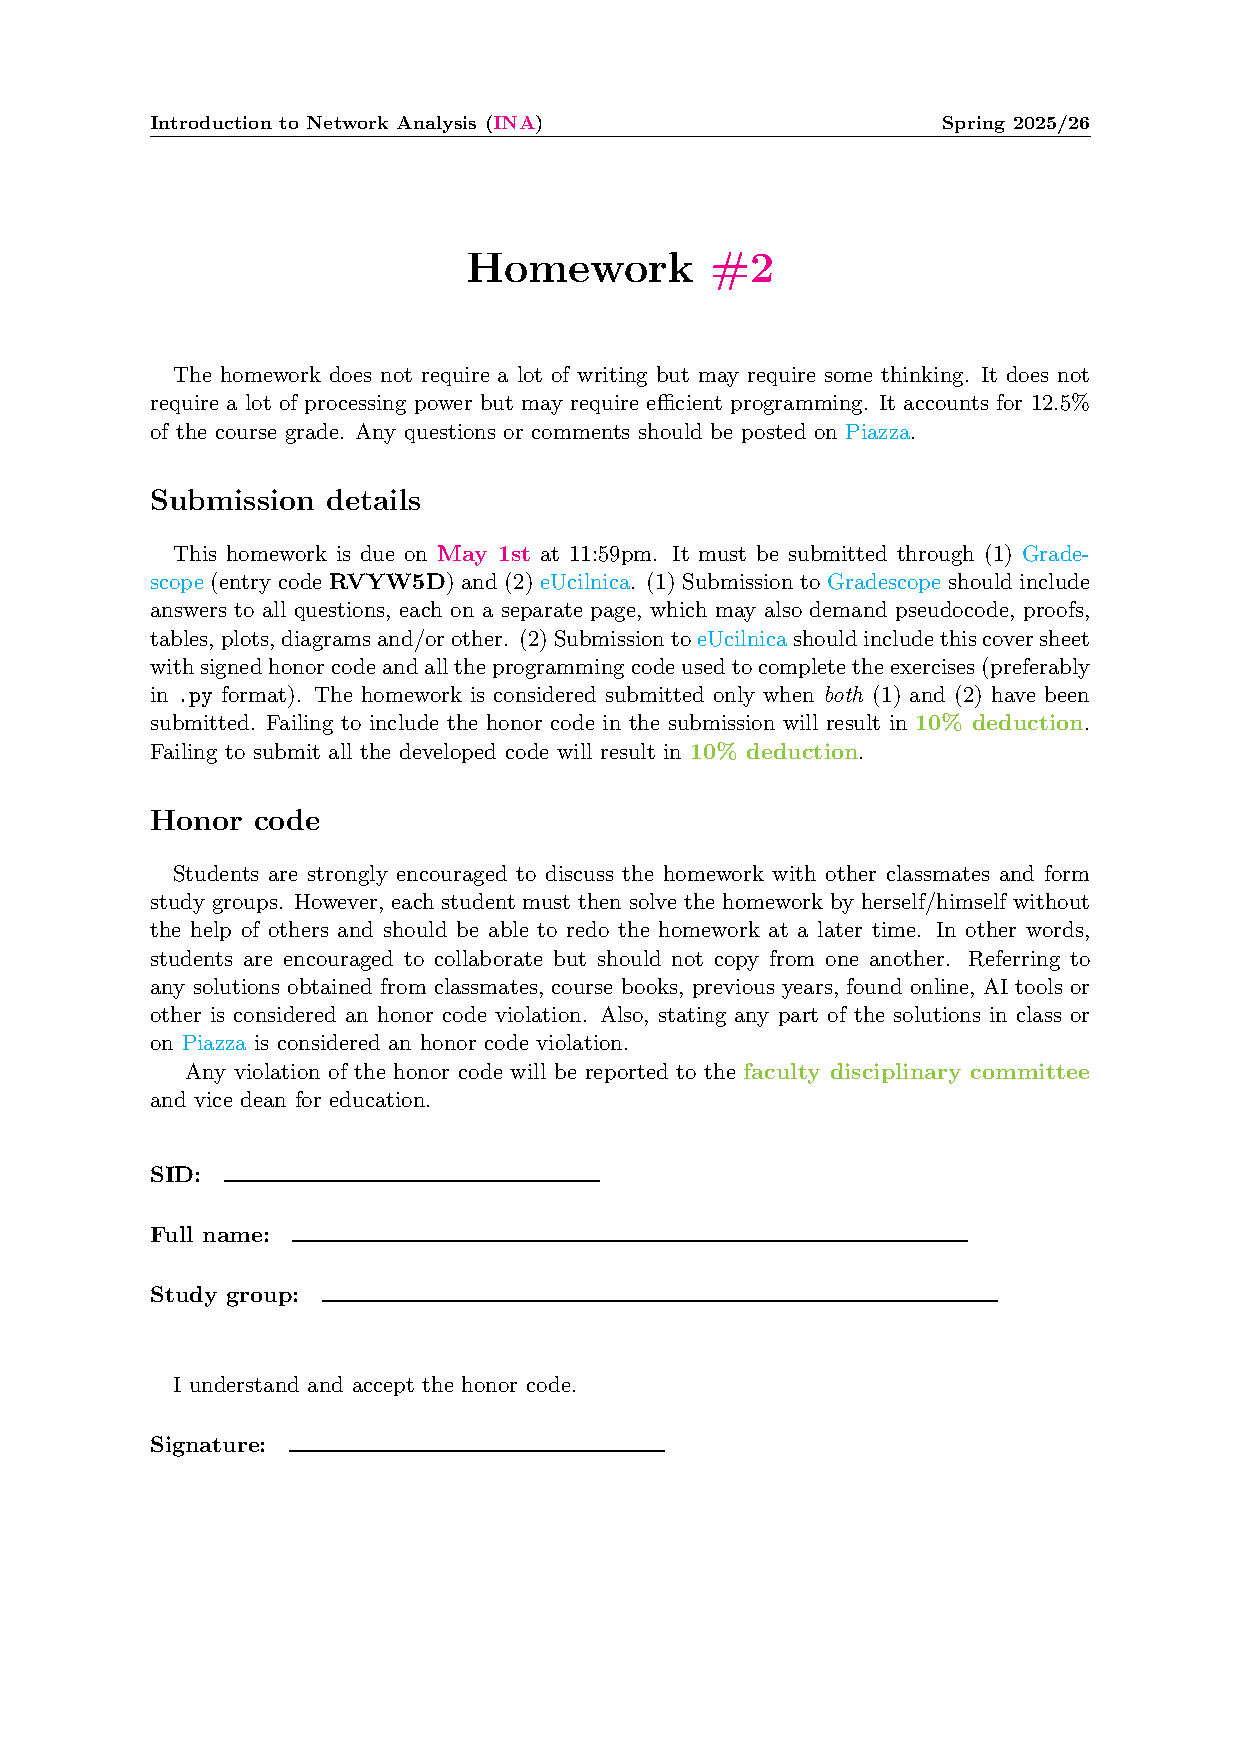
\includepdf[pages=1]{hw2.pdf}

\end{document}
